\documentclass[12pt,a4paper,utf8]{ctexart}
\usepackage{graphicx}
\usepackage{amsmath}
\usepackage{amssymb}
\usepackage{subfig}
\usepackage{cite}
\usepackage[ntheorem]{empheq}
\usepackage{enumitem}
\usepackage{fullpage}
\usepackage{cleveref}
\usepackage{cellspace}
\usepackage{listings}
\usepackage{color}
\usepackage{float}
\definecolor{gray}{rgb}{0.5,0.5,0.5}
\definecolor{dkgreen}{rgb}{.068,.578,.068}
\definecolor{dkpurple}{rgb}{.320,.064,.680}

% set Matlab styles
\lstset{
   language=Matlab,
   keywords={break,case,catch,continue,else,elseif,end,for,function,
      global,if,otherwise,persistent,return,switch,try,while},
   basicstyle=\ttfamily,
   keywordstyle=\color{blue}\bfseries,
   commentstyle=\color{dkgreen},
   stringstyle=\color{dkpurple},
   backgroundcolor=\color{white},
   tabsize=4,
   showspaces=false,
   breaklines,%自动换行
   showstringspaces=false,
   numbers=left,   % 行号的位置在左边
   columns=fixed,
}

\begin{document}
\CJKfamily{zhkai}


\begin{center}
   \textbf{作业二}\\
   \textbf{敖旭扬 ~~~~~ PB18071477 ~~~~~ \today}\\
\end{center}
\textit{}
\vspace{\baselineskip}

\begin{enumerate}
   \item[第一题] 解:本题均使用当前积分值与上一个计算出的积分值之差的绝对值$|I_n-I_{n-1}|<10^{-15}$作为结束计算的条件,即此时计算得到的积分值$I_n$已经是最精确的了。
         因为用Cauchy收敛准则可以证明$I_n$一定会收敛,且随着$n$增大,$|I_n-I_{n-1}|$也将减小,但是在双精度(double precision)的计算环境下,计算机的机器精度约为$2.22 \times 10^{−16}$。
         所以当$|I_n-I_{n-1}|<10^{-15}$时,由于计算机精度有限,$I_n$已经不能更精确了,它已经是最精确的了。
   \item[\textbf{(a)}]
         使用自动控制误差的复化梯形公式计算积分的\textsc{Matlab}程序显示如下:
         \lstinputlisting[frame=single]{src/p1a.m}

         上述程序在命令行输出的结果为:
         \begin{eqnarray}
            \begin{aligned}
               I & =1.339880713117284 \\
               n & =33554432
               \nonumber
            \end{aligned}
         \end{eqnarray}
         即在误差控制精度为$10^{-15}$的情况下,计算得最精确的结果为
         \begin{eqnarray}
            I=1.339880713117284
            \nonumber
         \end{eqnarray}
         上述程序输出的绝对误差随着迭代次数变化的semilogy图为:
         \begin{figure}[H]
            \centering
            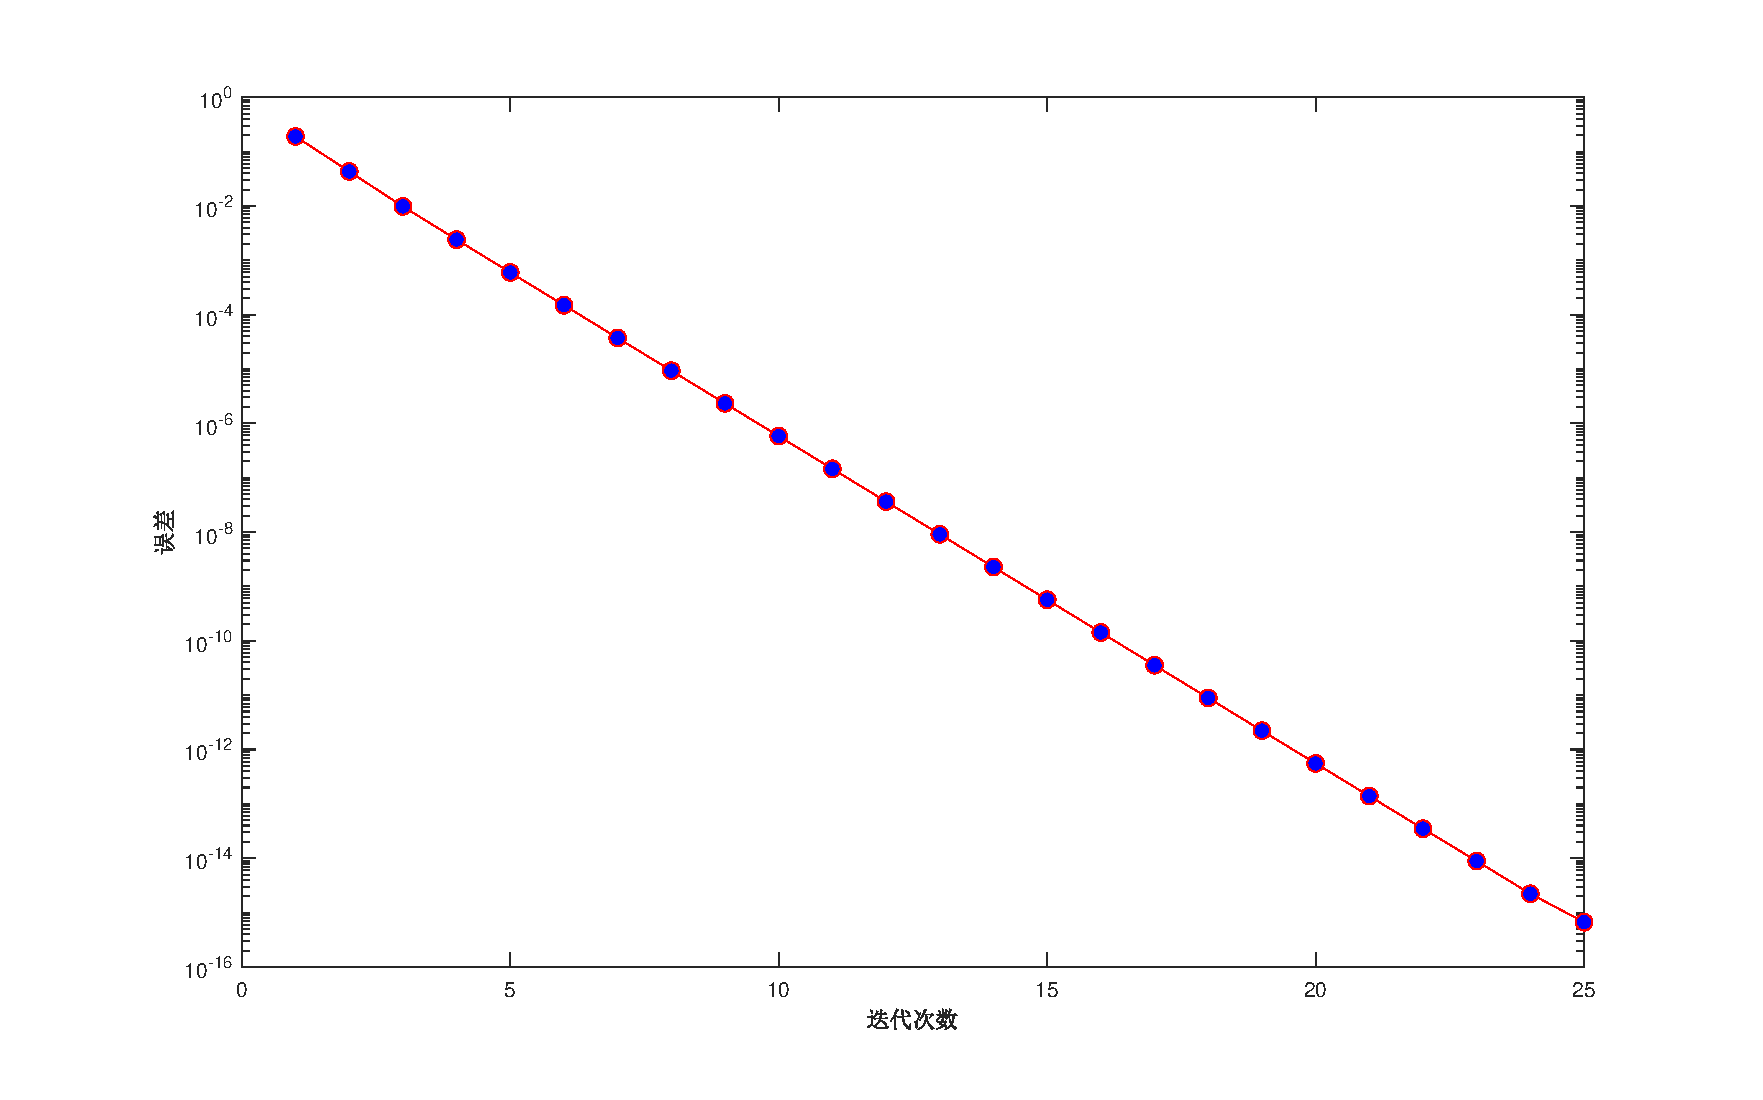
\includegraphics[width=1\textwidth]{fig/p1a.eps}
            \caption{使用自动控制误差的复化梯形公式的效果}
         \end{figure}

   \item[\textbf{(b)}]
         使用 Richardson 外推方法计算积分的\textsc{Matlab}程序显示如下:
         \lstinputlisting[frame=single]{src/p1b.m}

         上述程序在命令行输出的结果为:
         \begin{eqnarray}
            \begin{aligned}
               Irichardson & = 1.339880713117284 \\
               n           & =9
               \nonumber
            \end{aligned}
         \end{eqnarray}
         即在精度控制值为$10^{-15}$的情况下,计算得最精确的结果为
         \begin{eqnarray}
            I_{richardson}=1.339880713117284
            \nonumber
         \end{eqnarray}
         上述程序输出的绝对误差随着迭代次数变化的semilogy图为:
         \begin{figure}[H]
            \centering
            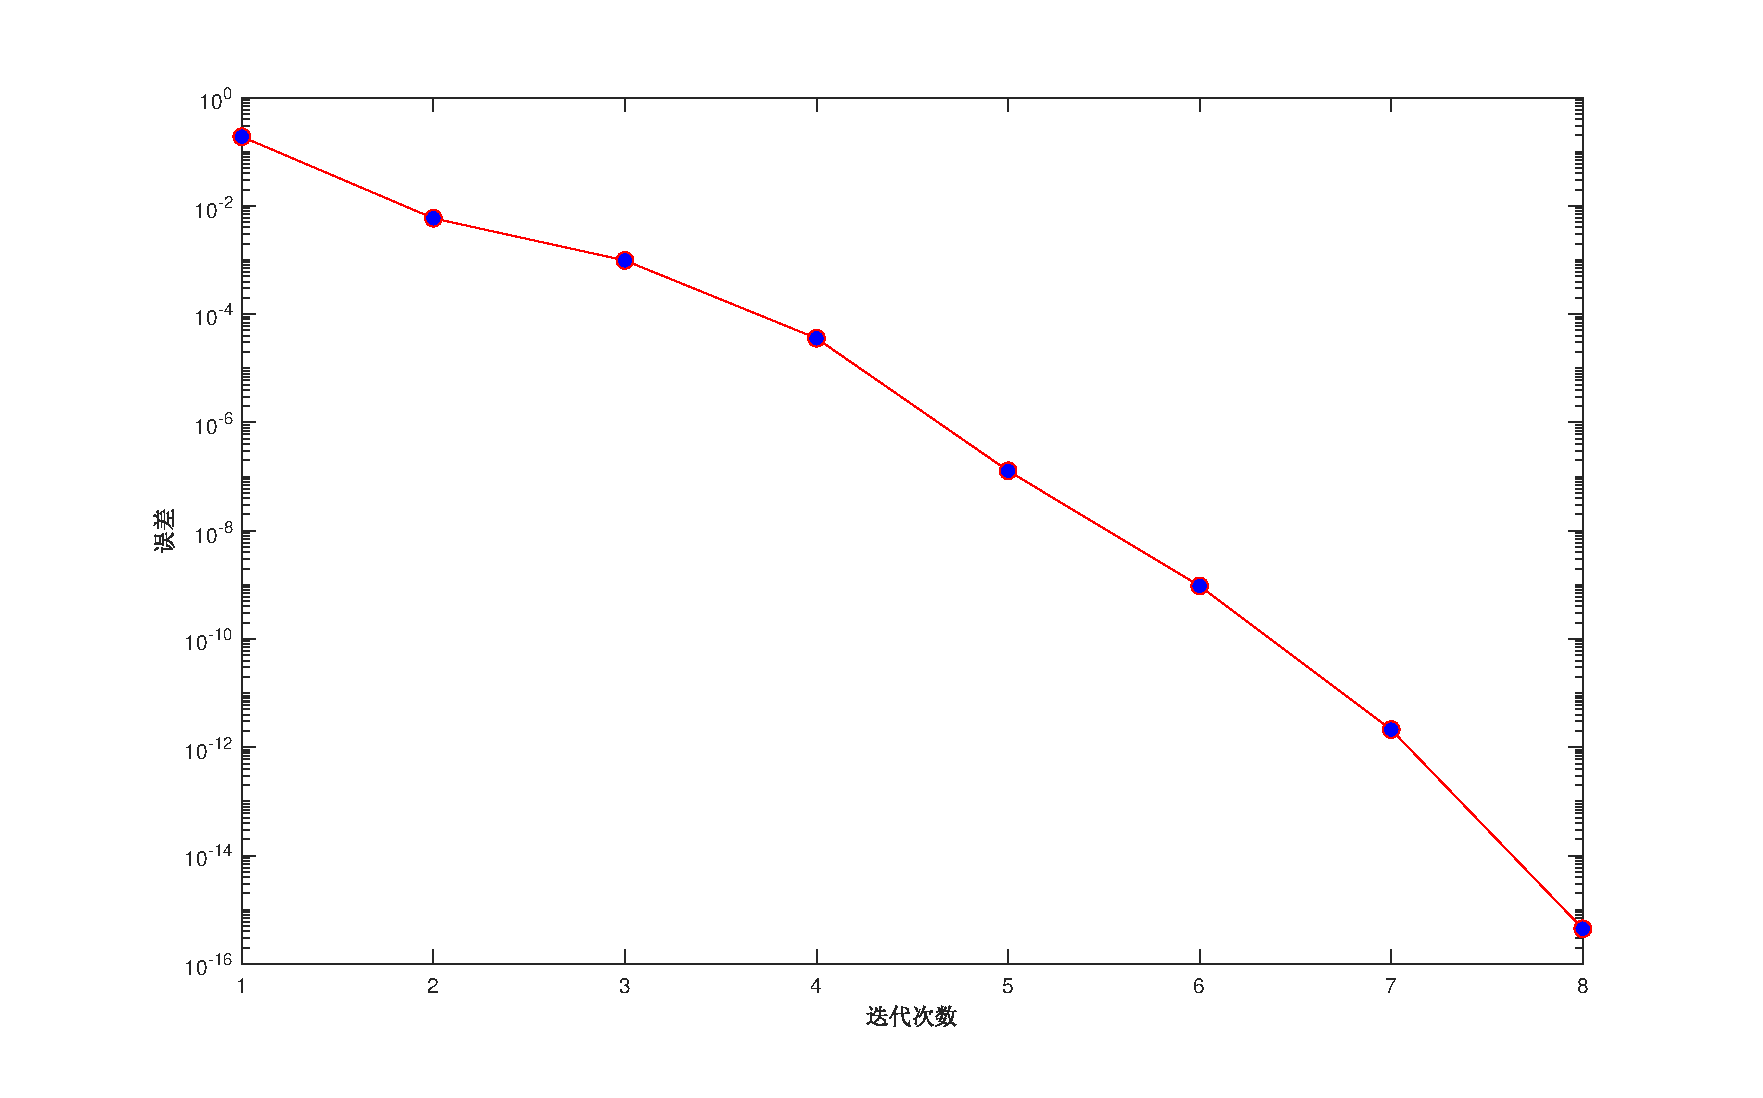
\includegraphics[width=1\textwidth]{fig/p1b.eps}
            \caption{使用Richardson外推方法的效果}
         \end{figure}

   \item[\textbf{(c)}]
         使用Gauß积分计算积分的\textsc{Matlab}程序显示如下:
         \lstinputlisting[frame=single]{src/p1c.m}

         上述程序在命令行输出的结果为:
         \begin{eqnarray}
            \begin{aligned}
               Igauss & =1.339880713117285 \\
               n      & =16
               \nonumber
            \end{aligned}
         \end{eqnarray}
         即在误差控制精度为$10^{-15}$的情况下,计算的最精确的结果为
         \begin{eqnarray}
            I_{gauss}=1.339880713117285
            \nonumber
         \end{eqnarray}
         上述程序输出的绝对误差随着迭代次数变化的semilogy图为:
         \begin{figure}[H]
            \centering
            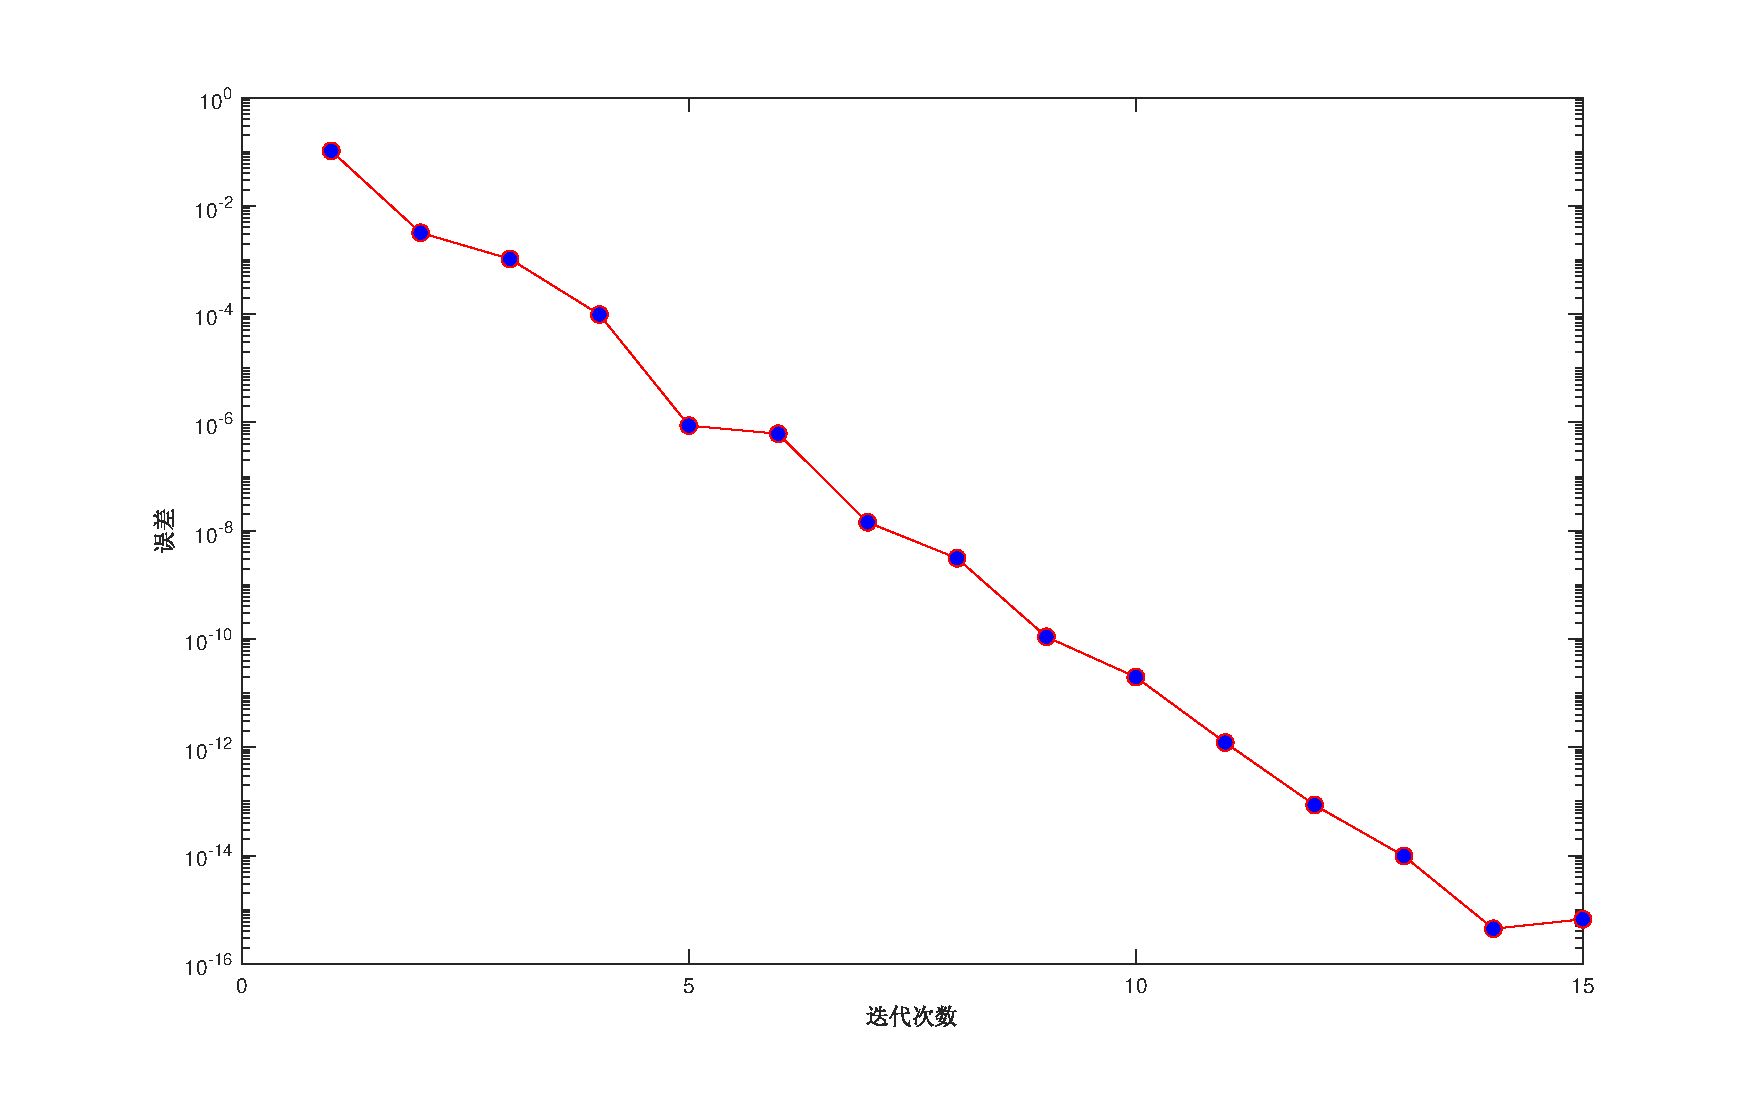
\includegraphics[width=1\textwidth]{fig/p1c.eps}
            \caption{使用Gauß积分的效果}
         \end{figure}

   \item[\textbf{(d)}]三种方法均使用自动误差控制逐步迭代来达到一个满意的最精确的结果:\\
         (a)中\textsc{Matlab}程序输出分点数为$n=33554432$,则使用自动控制误差的复化梯形公式的方法的采样点总数约为
         \begin{eqnarray}
            \begin{aligned}
               N_a=n=33554432
               \nonumber
            \end{aligned}
         \end{eqnarray}
         (b)中\textsc{Matlab}程序输出迭代次数为$n=9$,则使用Richardson外推方法的方法的采样点总数约为
         \begin{eqnarray}
            \begin{aligned}
               N_b=\sum_{k=2}^{n} 2^{k-2}=\sum_{i=0}^{n-2} 2^{i}=2^{n-1}-1=2^{9-1}-1=255
               \nonumber
            \end{aligned}
         \end{eqnarray}
         (c)中\textsc{Matlab}程序输出迭代次数为$n=16$,则使用Gauß积分的方法的采样点总数约为
         \begin{eqnarray}
            \begin{aligned}
               N_c=\sum_{k=1}^{n}k=\frac{n(n+1)}{2}=\frac{16(16+1)}{2}=136
               \nonumber
            \end{aligned}
         \end{eqnarray}
         综上所述,$N_c<N_b\ll N_a$,所以从取样总数考虑,三种方法的效率:(c)的效率高于(b)的效率,
         (b)、(c)的效率远高于(a)的效率。
   \item[第二题] 解:
   \item[\textbf{(a)}] 证明:\\
         由于
         \begin{eqnarray}
            \begin{aligned}
               \ell_j(x)=\frac{1}{\pi_j}\prod_{\substack{k=0 \\k \neq j}}^{n}(x-x_k)=\frac{e_j(x)}{\pi_j}
            \end{aligned}
         \end{eqnarray}
         其中
         \begin{eqnarray}
            \begin{aligned}
               e_j(x)=\prod_{\substack{k=0 \\k \neq j}}^{n}(x-x_k)
            \end{aligned}
         \end{eqnarray}
         而
         \begin{eqnarray}
            \begin{aligned}
               e_j'(x)=\sum_{\substack{t=0 \\ t\neq j}}^{n}\prod_{\substack{k=0\\k \neq t,j}}^{n}(x-x_k)
               =\sum_{\substack{k=0        \\k\neq j}}^{n}\frac{e_j(x)}{(x-x_k)}
               =e_j(x)\sum_{\substack{k=0  \\k\neq j}}^{n}(x-x_k)^{-1}
            \end{aligned}
         \end{eqnarray}
         所以
         \begin{eqnarray}
            \begin{aligned}
               \ell_j'(x)=\Big(\frac{e_j(x)}{\pi_j}\Big)'=\frac{e_j'(x)}{\pi_j}=
               \frac{e_j(x)}{\pi_j}\sum_{\substack{k=0 \\k\neq j}}^{n}(x-x_k)^{-1}
               =\ell_j(x)\sum_{\substack{k=0           \\k\neq j}}^{n}(x-x_k)^{-1}
            \end{aligned}
         \end{eqnarray}
         则
         \begin{eqnarray}
            \begin{aligned}
               p'(x)=\sum_{j=0}^{n}f_j\ell_j'(x)=
               \sum_{j=0}^{n}\Biggl(f_j\ell_j(x)\sum_{\substack{k=0 \\k\neq j}}^{n}(x-x_k)^{-1} \Biggr)
            \end{aligned}
         \end{eqnarray}
   \item[\textbf{(b)}]
         用等距插值计算$f(x)=\sin(x)$在$[-1,1]$上的导数的\textsc{Matlab}程序显示如下:
         \lstinputlisting[frame=single]{src/p2b.m}
         上述程序输出的计算出的导函数与真实解$f'(x)=\cos(x)$的图像为:
         \begin{figure}[H]
            \centering
            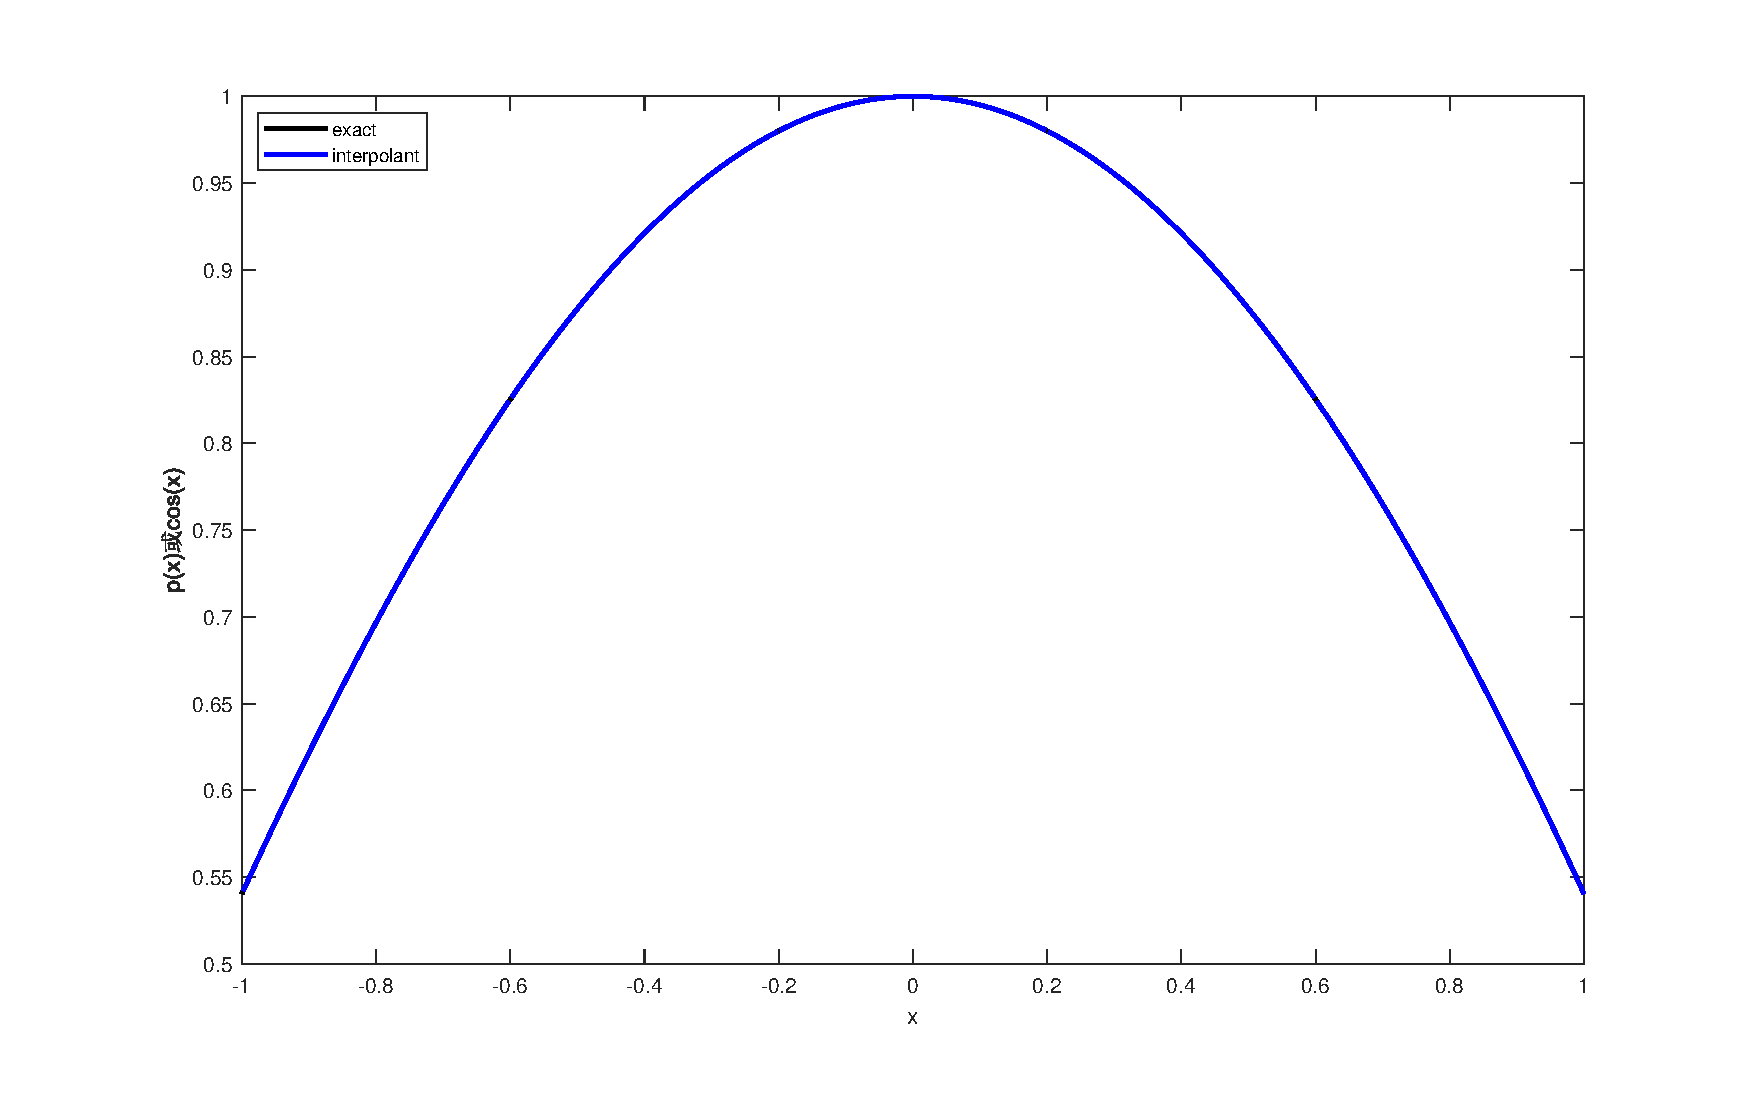
\includegraphics[width=1\textwidth]{fig/p2b1.eps}
            \caption{导函数图像}
         \end{figure}
         逐点误差绝对值的semilogy图为:
         \begin{figure}[H]
            \centering
            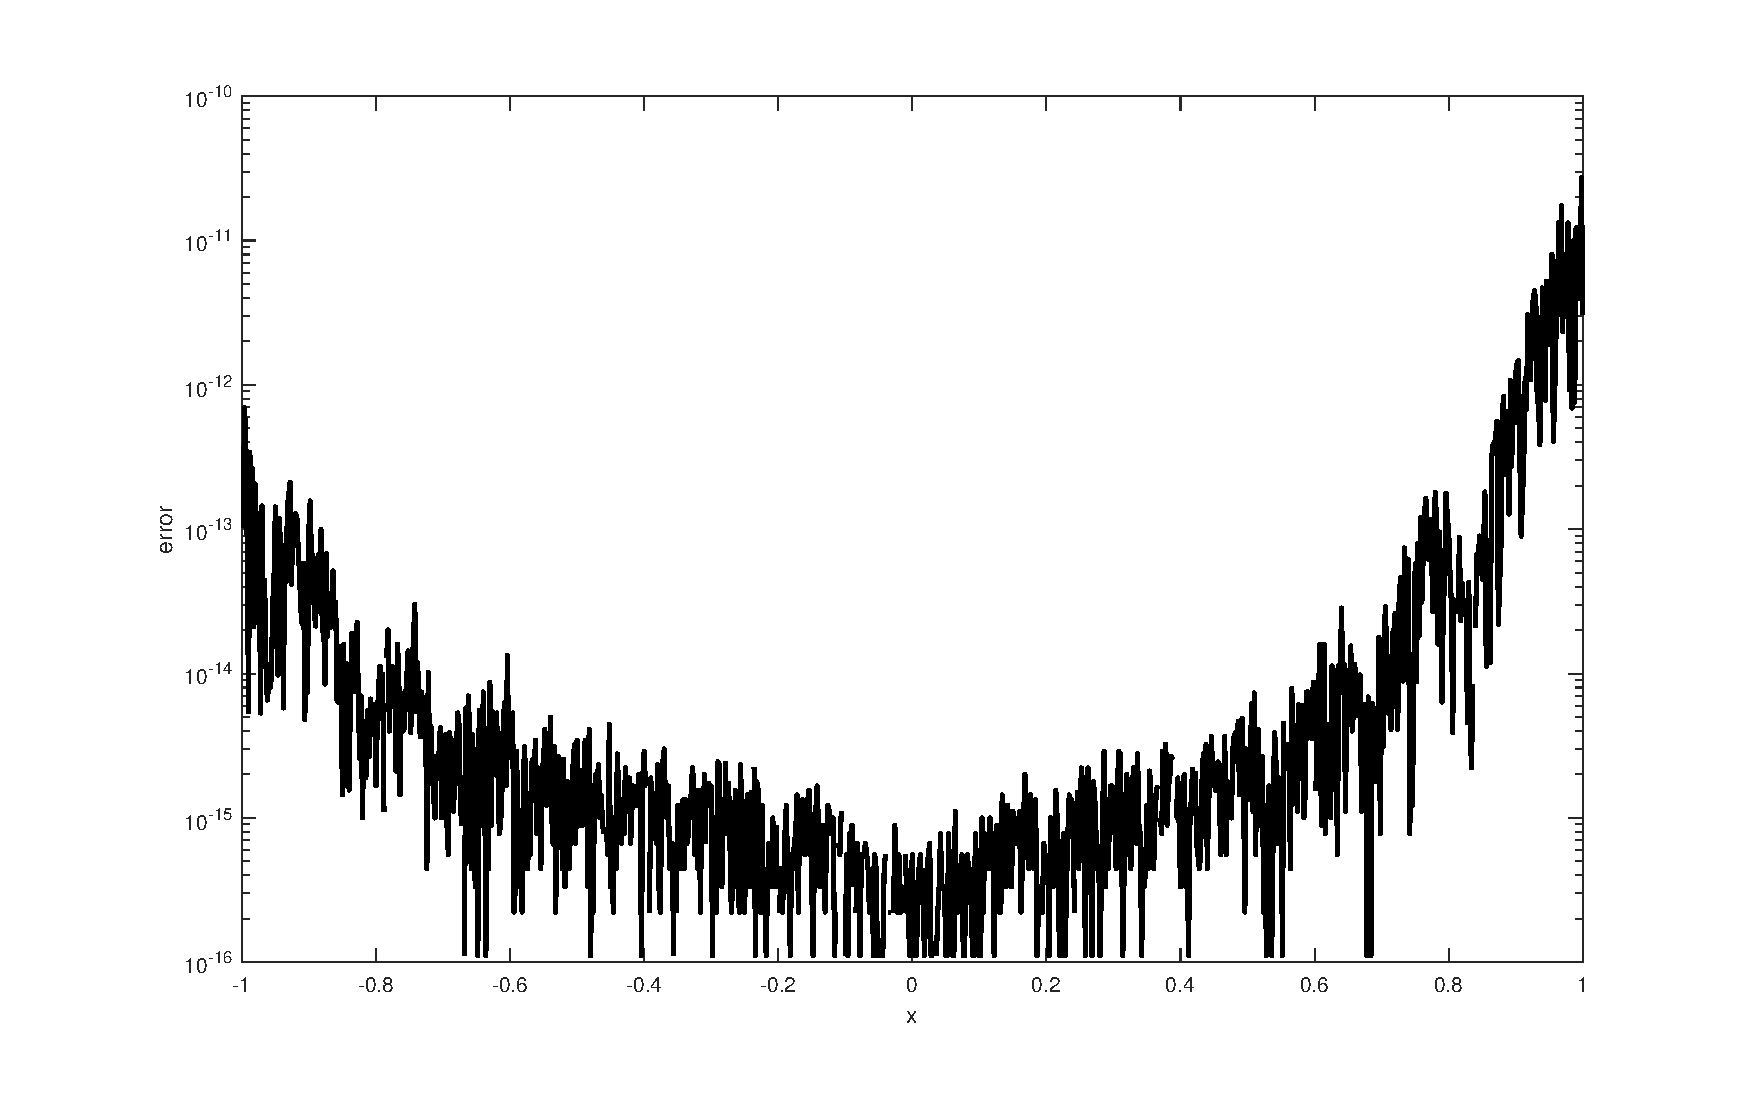
\includegraphics[width=1\textwidth]{fig/p2b2.eps}
            \caption{逐点误差的绝对值}
         \end{figure}
   \item[\textbf{(c)}] 证明:\\
         由
         \begin{eqnarray}
            \begin{aligned}
               \boldsymbol{p}'=\boldsymbol{Df}
            \end{aligned}
         \end{eqnarray}
         得
         \begin{eqnarray}
            \begin{aligned}
               p'(x_i)=\sum_{j=0}^{n}f_jD_{ij}
            \end{aligned}
         \end{eqnarray}
         又由$(5)$式,有
         \begin{eqnarray}
            \begin{aligned}
               D_{ij}=\ell_j(x_i)\sum_{\substack{k=0 \\ k\neq j}}^{n}(x_i-x_k)^{-1}
            \end{aligned}
         \end{eqnarray}
         又
         \begin{eqnarray}
            \begin{aligned}
               \ell_j(x_k)=\begin{cases}1 &k=j \cr 0 &k \neq j \end{cases}
            \end{aligned}
         \end{eqnarray}
         所以$i = j$时
         \begin{eqnarray}
            \begin{aligned}
               D_{ij}=\ell_j(x_i)\sum_{\substack{k=0 \\ k\neq j}}^{n}(x_i-x_k)^{-1}
               =\sum_{\substack{k=0                  \\ k\neq j}}^{n}(x_i-x_k)^{-1}
            \end{aligned}
         \end{eqnarray}
         而$i \neq j$时,根据$(5)$式前一个等式部分
         \begin{eqnarray}
            \begin{aligned}
               D_{ij}=\ell_j'(x_i)=\ell_j'(x)\Big|_{x=x_i}=\frac{1}{\pi_j}e_j'(x)\Big|_{x=x_i}
            \end{aligned}
         \end{eqnarray}
         由$(3)$式得
         \begin{eqnarray}
            \begin{aligned}
               e_j'(x)\Big|_{x=x_i}=\sum_{\substack{t=0 \\ t\neq j}}^{n}\prod_{\substack{k=0\\k \neq t,j}}^{n}(x-x_k)\Big|_{x=x_i}
               =\sum_{\substack{t=0                     \\ t\neq j}}^{n}\prod_{\substack{k=0\\k \neq t,j}}^{n}(x_i-x_k)
               =\prod_{\substack{k=0                    \\k \neq i,j}}^{n}(x_i-x_k)
            \end{aligned}
         \end{eqnarray}
         所以$i \neq j$时
         \begin{eqnarray}
            \begin{aligned}
               D_{ij}=\frac{1}{\pi_j}e_j'(x)\Big|_{x=x_i}=\frac{1}{\pi_j}\prod_{\substack{k=0 \\k \neq i,j}}^{n}(x_i-x_k)
               =\frac{\pi_i}{\pi_j(x_i-x_j)}
            \end{aligned}
         \end{eqnarray}
         综上,有
         \begin{eqnarray}
            \begin{aligned}
               D_{ij}=
               \begin{cases}
                  \dfrac{1}{\pi_j}\prod\limits_{\substack{k=0 \\k \neq i,j}}^{n}(x_i-x_k)=\dfrac{\pi_i}{\pi_j(x_i-x_j)} & i \neq j \cr
                  \sum\limits_{\substack{k=0                  \\ k\neq j}}^{n}(x_i-x_k)^{-1} & i=j
               \end{cases}
            \end{aligned}
         \end{eqnarray}
   \item[\textbf{(d)}]
         \textsc{Matlab}程序显示如下:
         \lstinputlisting[frame=single]{src/p2d.m}
         上述程序输出的图像为:
         \begin{figure}[H]
            \centering
            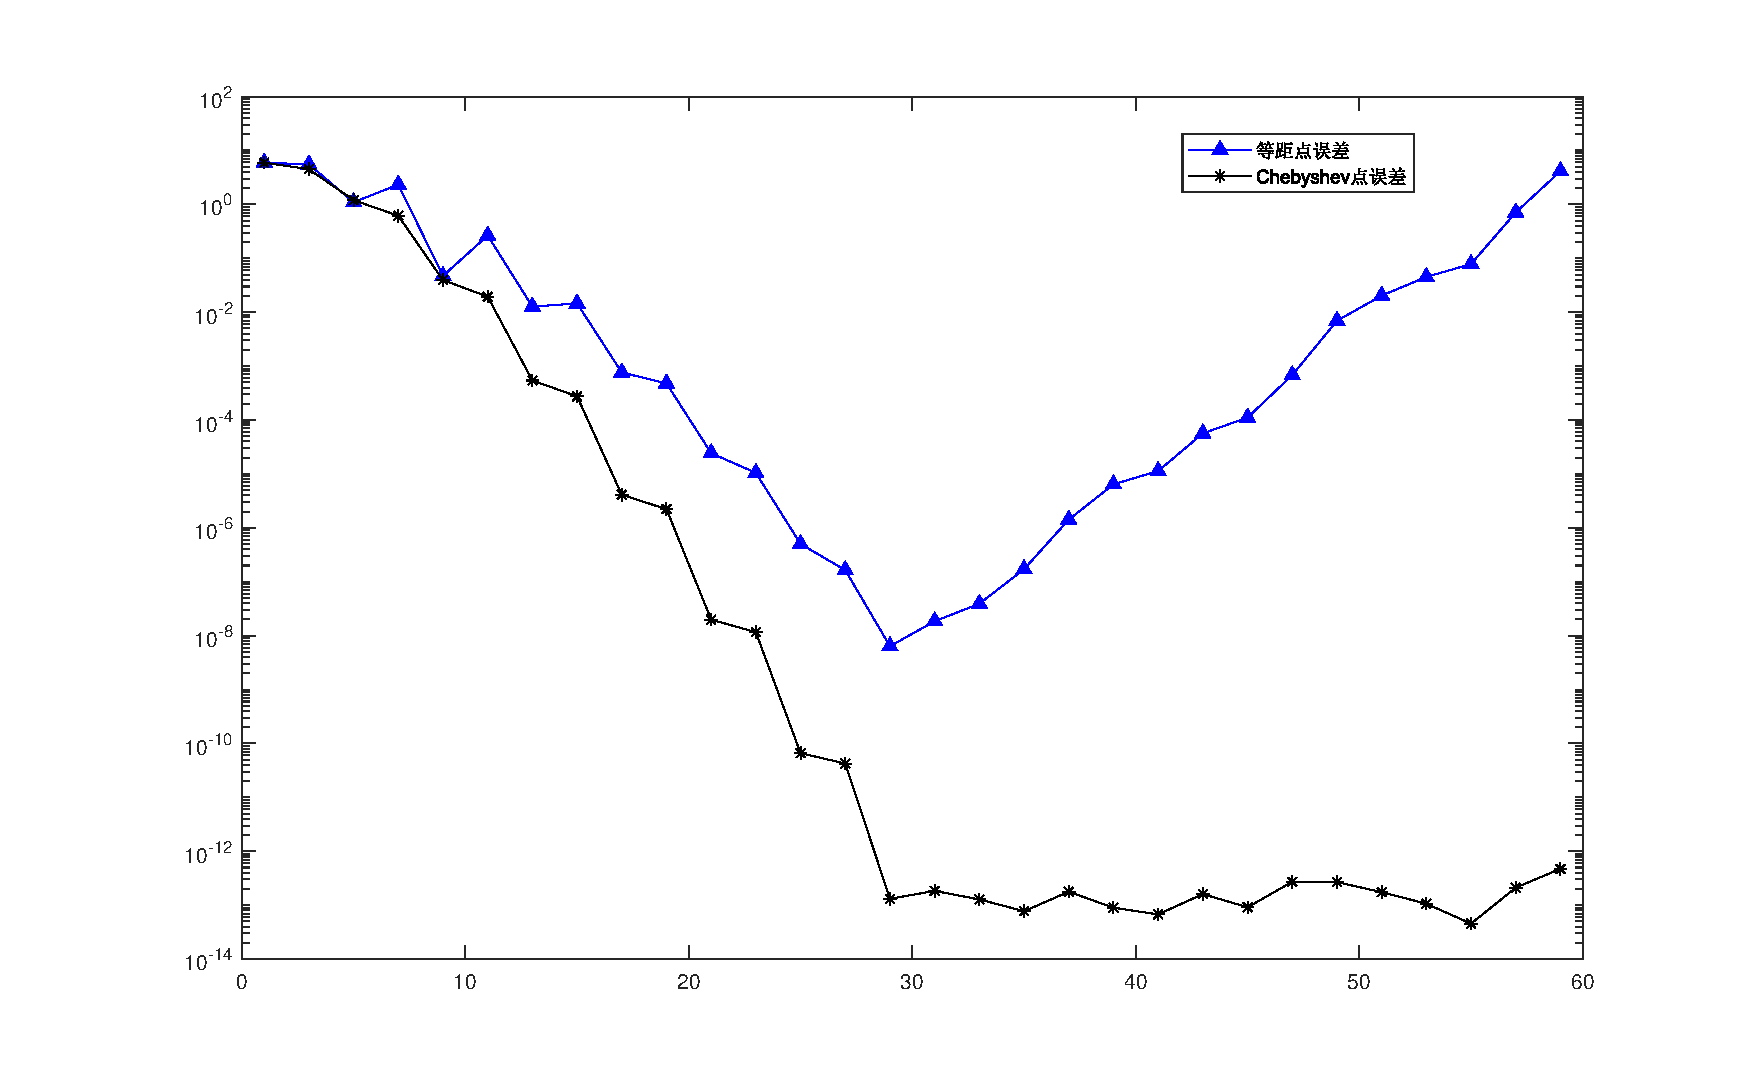
\includegraphics[width=1\textwidth]{fig/p2d.eps}
            \caption{等距点和Chebyshev点上的误差绝对值}
         \end{figure}
         观察发现,使用Chebyshev点时,在最大误差下降到$10^{-13}$之后就基本保持(同一数量级)不变了;而使用等距点时,
         $n=29$时最大误差下降到最小值,之后却一直增大,甚至到$n=59$时,最大误差高达$4.139913901026180$。这是因为出现了Runge(龙格)现象,
         高次多项式的插值效果不一定优于低次多项式的插值的效果,同时等距插值不能保证有较好的插值效果。
   \item[第三题]
   \item[\textbf{(a)}]该多步法公式中的系数为
         \begin{eqnarray}
            \begin{aligned}
               \alpha & =\int_{x_{n-1}}^{x_{n+1}}\dfrac{(x-x_{n})(x-x_{n-1})(x-x_{n-2})}{(x_{n+1}-x_{n})(x_{n+1}-x_{n-1})(x_{n+1}-x_{n-2})}\mathrm{d}x=\dfrac{h}{3} \\
               \beta  & =\int_{x_{n-1}}^{x_{n+1}}\dfrac{(x-x_{n+1})(x-x_{n-1})(x-x_{n-2})}{(x_{n}-x_{n+1})(x_{n}-x_{n-1})(x_{n}-x_{n-2})}\mathrm{d}x=\dfrac{4h}{3}  \\
               \gamma & =\int_{x_{n-1}}^{x_{n+1}}\dfrac{(x-x_{n+1})(x-x_{n})(x-x_{n-2})}{(x_{n-1}-x_{n+1})(x_{n-1}-x_{n})(x_{n-1}-x_{n-2})}\mathrm{d}x=\dfrac{h}{3} \\
               \mu    & =\int_{x_{n-1}}^{x_{n+1}}\dfrac{(x-x_{n+1})(x-x_{n})(x-x_{n-1})}{(x_{n-2}-x_{n+1})(x_{n-2}-x_{n})(x_{n-2}-x_{n-1})}\mathrm{d}x=0
               \nonumber
            \end{aligned}
         \end{eqnarray}
   \item[\textbf{(b)}]截断为
         \begin{eqnarray}
            \begin{aligned}
               T_{n+1}&=\int_{x_{n-1}}^{x_{n+1}}R(x)\mathrm{d}x
               =\int_{x_{n-1}}^{x_{n+1}}\dfrac{y^{(5)}(\xi )}{5!}(x-x_{n+1})(x-x_{n})(x-x_{n-1})(x-x_{n-2})\mathrm{d}x\\
               &=\dfrac{y^{(5)}(\xi )}{5!}\int_{x_{n-1}}^{x_{n+1}}(x-x_{n+1})(x-x_{n})(x-x_{n-1})(x-x_{n-2})\mathrm{d}x\\
               &=\dfrac{y^{(5)}(\xi )}{5!}\cdot \dfrac{-4h^5}{15}=-\dfrac{1}{450}h^5y^{(5)}(\xi )=O(h^{5})=O(h^{4+1})
               \nonumber
            \end{aligned}
         \end{eqnarray}
         所以此格式是$4$阶的。
   \item[\textbf{(c)}]由(a)得到计算格式
   \begin{eqnarray}
      \begin{aligned}
         y_{n+1}=y_{n-1}+\dfrac{h}{3}(f_{n-1}+4f_{n}+f_{n+1})
         \nonumber
      \end{aligned}
   \end{eqnarray}
   代入
   \begin{eqnarray}
      \begin{aligned}
         f_n=f(x_n,y_n)=x_{n}e^{-5x_{n}}-5y_{n}
         \nonumber
      \end{aligned}
   \end{eqnarray}
   得
   \begin{eqnarray}
      \begin{aligned}
         y_{n+1}=y_{n-1}+\dfrac{h}{3}[x_{n-1}e^{-5x_{n-1}}-5y_{n-1}+4(x_{n}e^{-5x_{n}}-5y_{n})+x_{n+1}e^{-5x_{n+1}}-5y_{n+1}]
         \nonumber
      \end{aligned}
   \end{eqnarray}
   令$g_n=x_ne^{-5x_n}$,整理得到下面的递归计算式
   \begin{eqnarray}
      \begin{aligned}
         y_{n+1}=\dfrac{y_{n-1}+\dfrac{h}{3}\Big[g_{n-1}-5y_{n-1}+4g_{n}-20y_{n}+g_{n+1}\Big]}{1+\frac{5h}{3}}
      \end{aligned}
   \end{eqnarray}
   所以可以用三阶Runge-Kutta方法起步计算出前两项,再用上式计算出其后所有项,求解的\textsc{Matlab}程序显示如下:
   \lstinputlisting[frame=single]{src/p3c.m}
   上述程序输出的图像为:
   \begin{figure}[H]
      \centering
      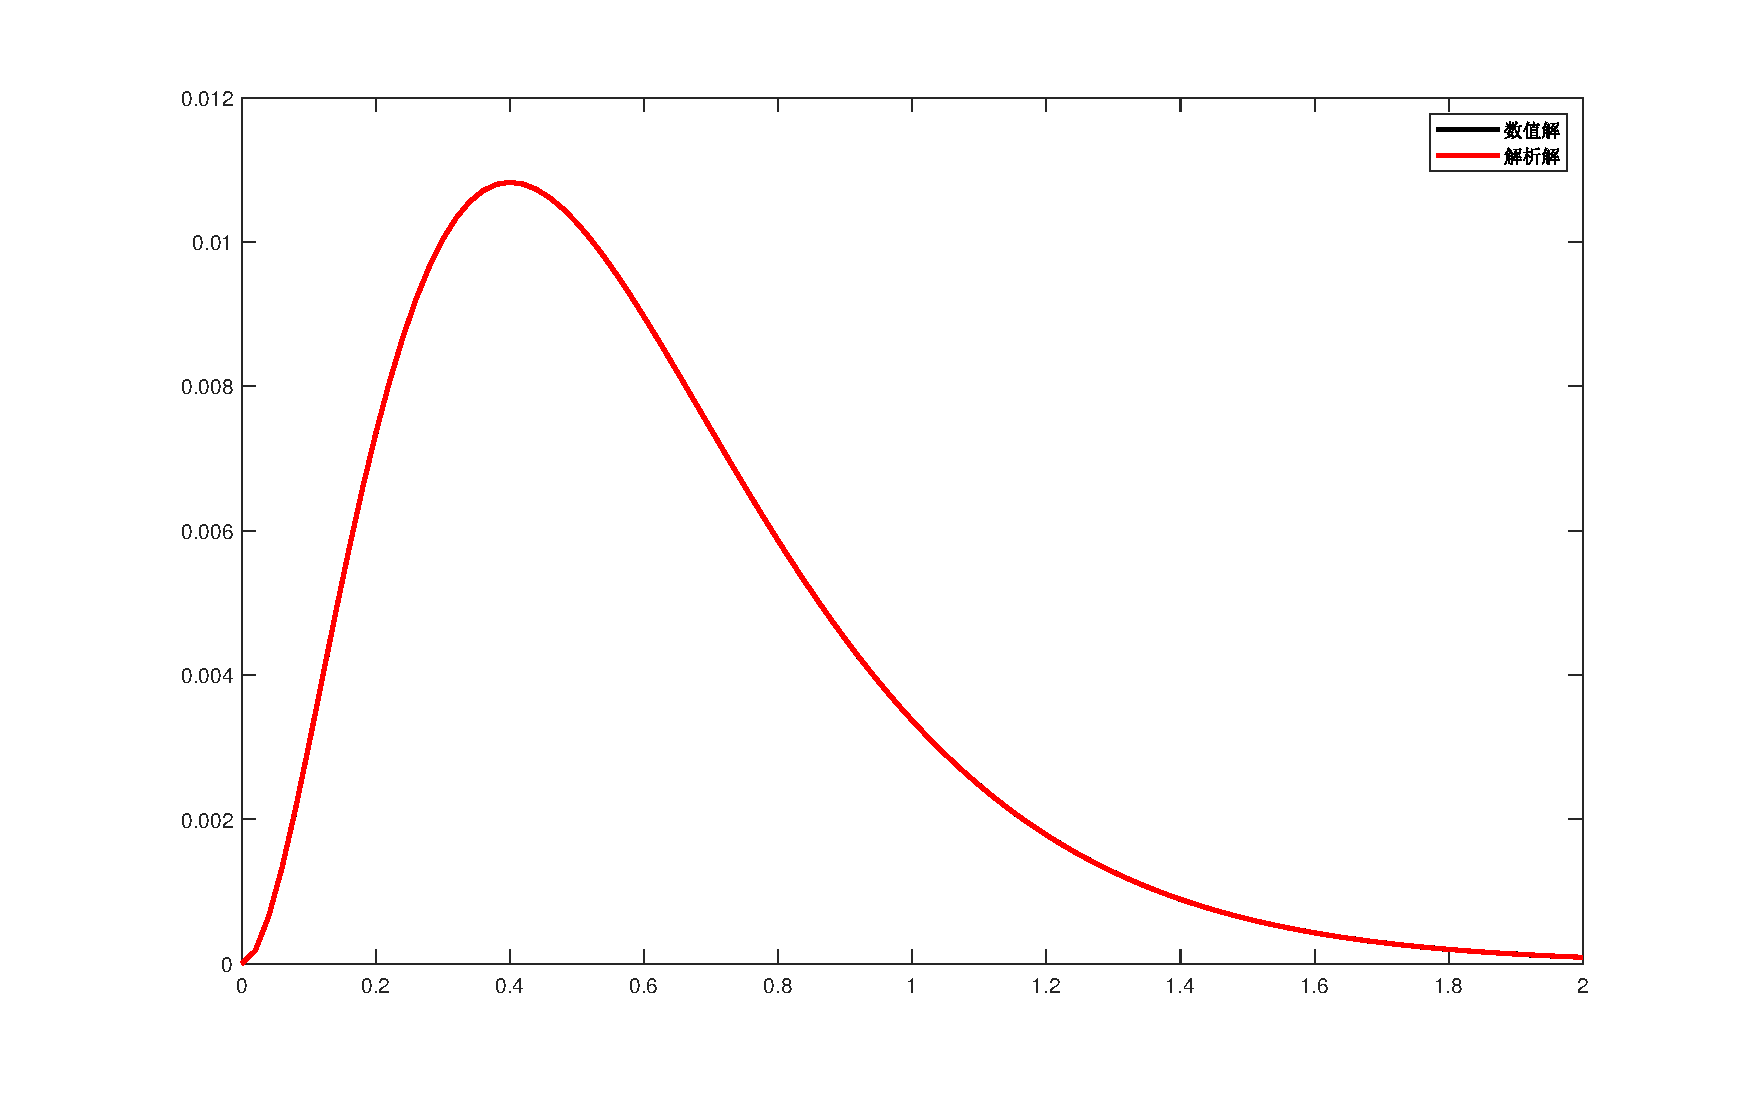
\includegraphics[width=1\textwidth]{fig/p3c.eps}
      \caption{Runge-Kutta方法起步和线性多步法求解初值问题的结果}
   \end{figure}
   可以看到数值解与解析解完全重合,三阶的Runge-Kutta方法作为三阶格式之所以不会影响使用该多步法时的精度,是因为
   三阶的Runge-Kutta方法局部截断误差为$O(h^4)$,而多步法的局部截断误差为$O(h^5)$,
   满足“起步计算的格式的精度至多只能比该格式的精度低一阶”的条件,所以不会影响求解精度。
   \item[\textbf{(d)}]一阶常微分方程有如下求解公式
   \begin{eqnarray}
      \begin{aligned}
         y'+P(x)y=Q(x)
         \Rightarrow 
         y=e^{-\int P\mathrm{d}x}\Big[ \int{e^{-\int P\mathrm{d}x}Q(x)}\mathrm{d}x+C \Big]
         \nonumber
      \end{aligned}
   \end{eqnarray}
   所以对于所求的方程,即$P(x)=5,\quad Q(x)=xe^{-5x}$,代入上面的求解公式得精确解为
   \begin{eqnarray}
      \begin{aligned}
         y=\dfrac{1}{2}x^2e^{-5x}
      \end{aligned}
   \end{eqnarray}
   取一系列$n$值或$h$值,计算出相应的数值解和精确解误差的最大值,再将这一系列误差最大值和$h$值画成loglog图,
   求解的\textsc{Matlab}程序显示如下:
   \lstinputlisting[frame=single]{src/p3d.m}
   上述程序输出的图像为:
   \begin{figure}[H]
      \centering
      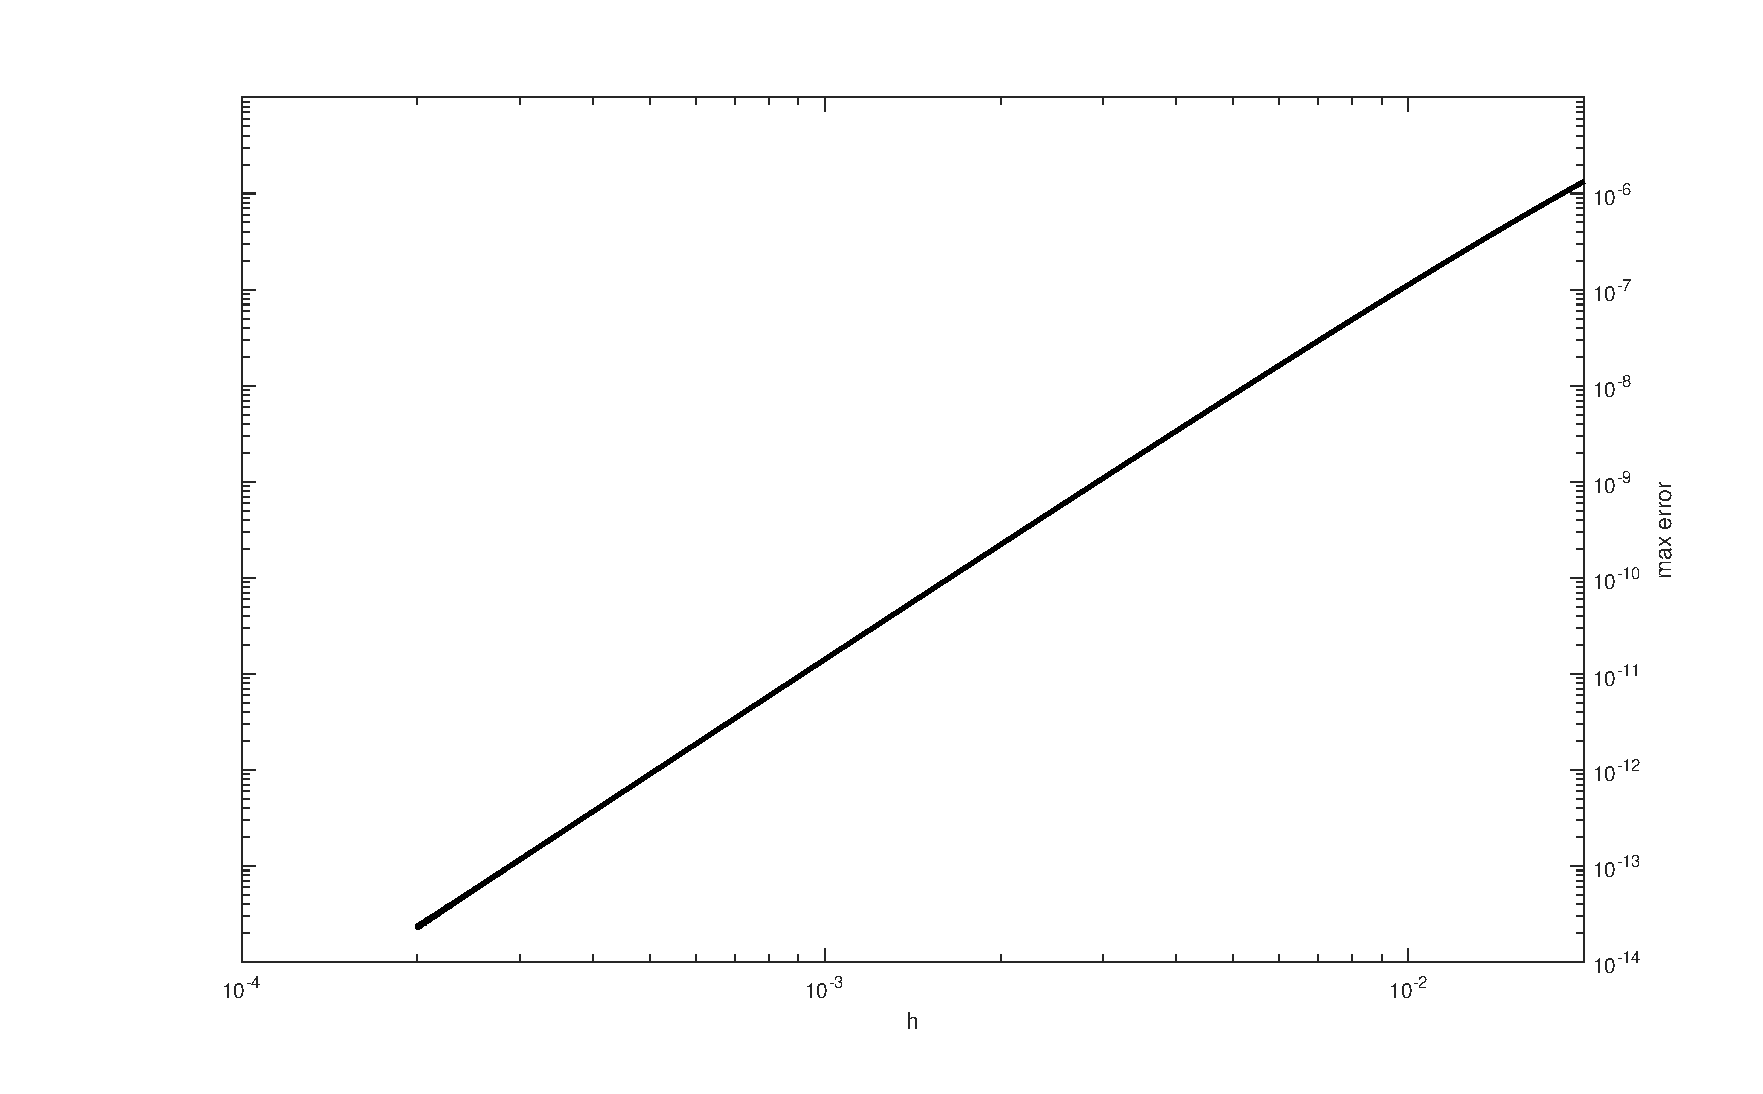
\includegraphics[width=1\textwidth]{fig/p3d.eps}
      \caption{线性多步法求解初值问题的误差和步长的loglog图}
   \end{figure}
   可以看到误差和步长$h$的对数斜率约为$4$,这就证实了(b)中推断的阶数$4$是正确的,此格式的整体截断误差为$O(h^4)$。
\end{enumerate}

\end{document}
